\documentclass[oneside]{book}
\usepackage{epsfig,graphicx} % Required for inserting images
\usepackage{amsmath}
\usepackage{amsthm}
\usepackage{amssymb}
\usepackage{subcaption}
\usepackage[spanish,mexico]{babel}
\usepackage[bookmarksopen]{hyperref}
\usepackage[utf8]{inputenc}
\usepackage{array}
\usepackage{listings} %Soporte para código
\usepackage[left=2cm,right=2cm,top=1.8cm,bottom=2.3cm]{geometry}
% ---definición de los paquetes--
\usepackage{fancyhdr}            % Permits header customization. See header section below.
\fancypagestyle{plain}{
    \lhead{}
    \fancyhead[R]{\thepage}
    \fancyhead[L]{}
    \renewcommand{\headrulewidth}{0pt}
    \fancyfoot{}
}
\pagestyle{fancy}
\fancyhead[R]{\thepage}
\fancyhead[L]{}
\title{Tarea 01: Naturales, inducción y recursión}
\author{Ramírez Mendoza Joaquín Rodrigo\\
Villalobos Juárez Gontran Eliut\\
Treviño Puebla Héctor Jerome}
\date{\today}
% ---Inicio de la portada
\begin{document}

    \begin{titlepage}

    \begin{minipage}{3cm}
    	\begin{center}
    		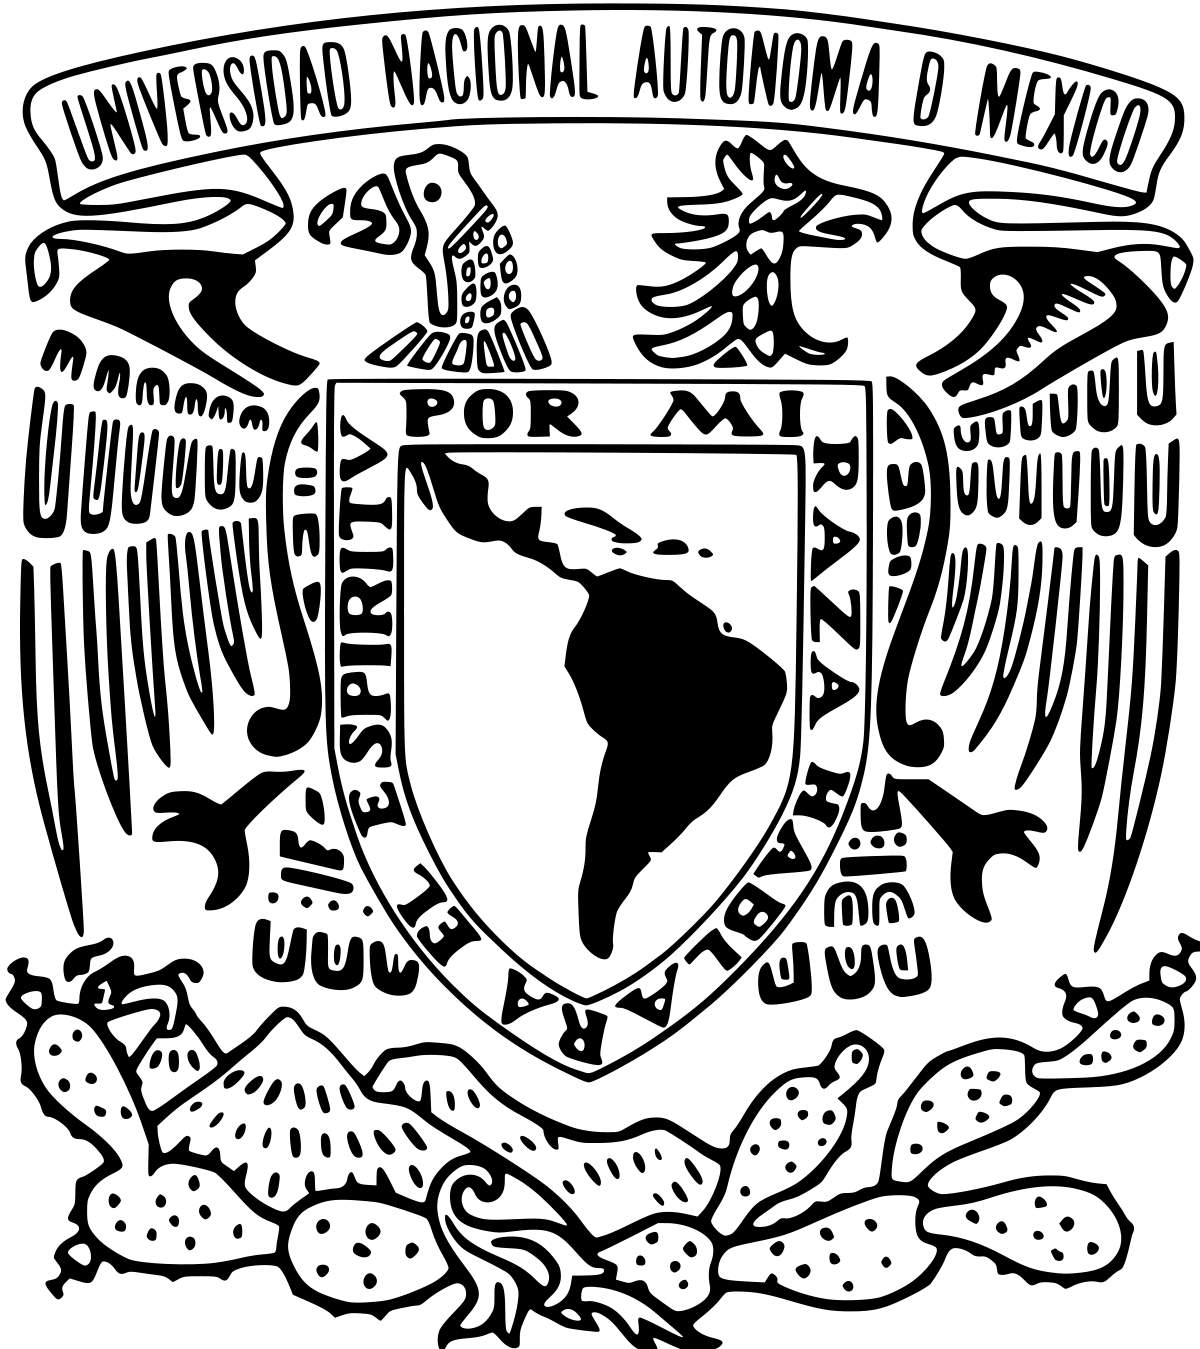
\includegraphics[height = 0.14\textheight]{recursos/Logo_UNAM.png}\par
    	\end{center}
    \end{minipage}\hfill
    \begin{minipage}{10cm}
    	
    \end{minipage}\hfill
    \begin{minipage}{3cm}
    	\begin{center}
    		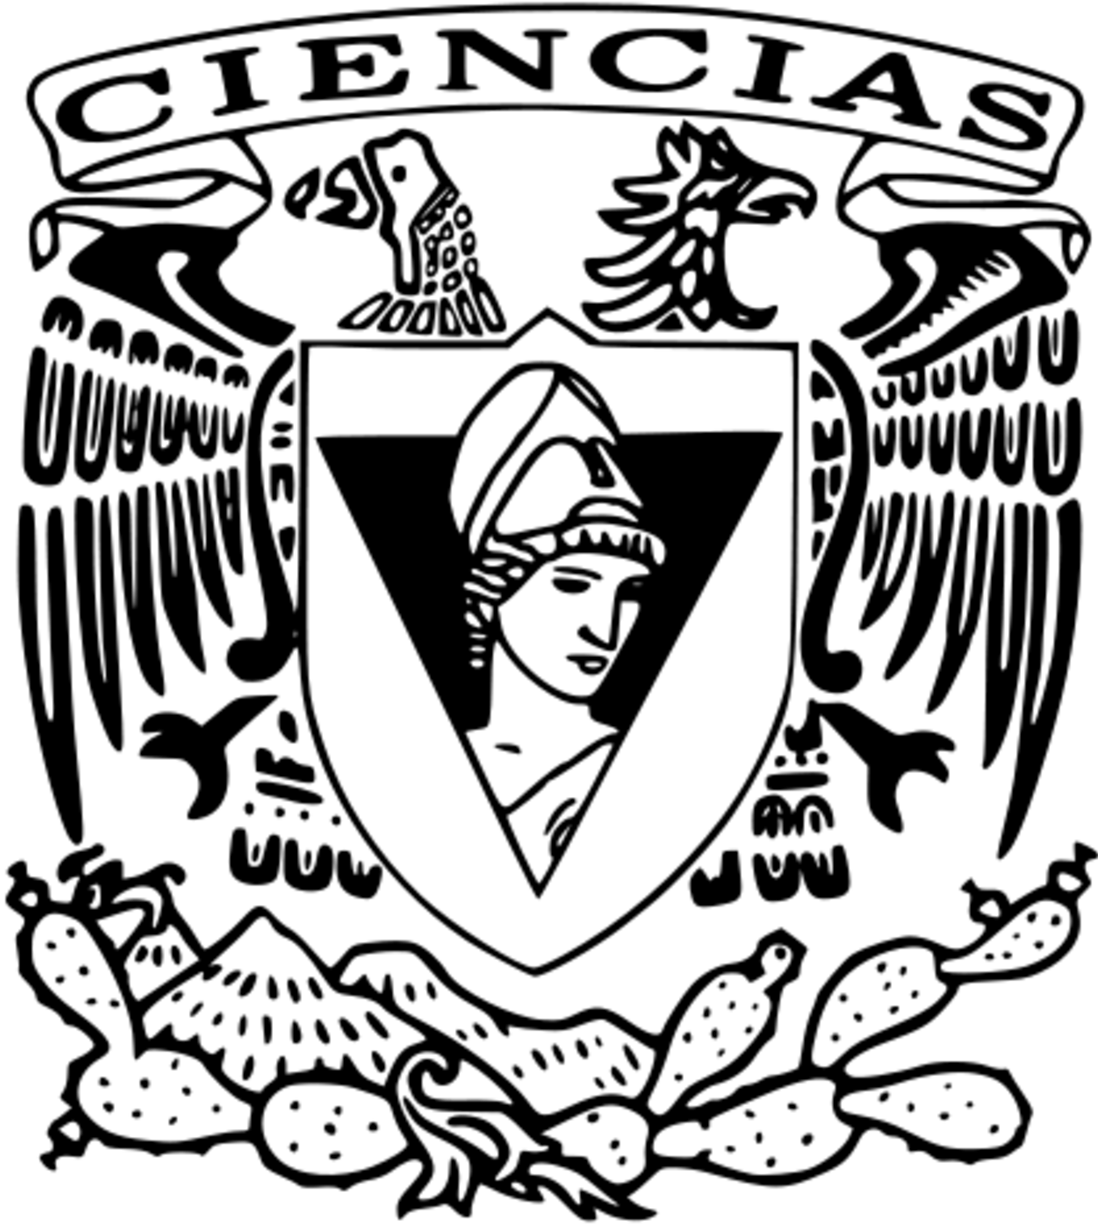
\includegraphics[height = 0.14\textheight]{recursos/Logo_FC.png}\par
    	\end{center}
    \end{minipage}
        \centering
        \vspace{1cm}
        
        {\bfseries\LARGE Universidad Nacional Autónoma de México \par}
        
        \vspace{1cm}
        {\scshape\Large Facultad de Ciencias \par}
        \vspace{1cm}
        {\scshape\Large Estructuras Discretas \par}
        \vspace{1cm}
        {\scshape\Large Licenciatura en Ciencias de la Computación \par}
        \vspace{1cm}
        {\scshape\Huge Tarea 01: Naturales, inducción y recursión.  \par}
        \vspace{3cm}
        {\itshape\Large Primer Parcial \par}
        \vfill
        {\Large Autores: \par}
        {\Large Ramírez Mendoza Joaquín Rodrigo \par}
        {\Large Villalobos Juárez Gontran Eliut\par}
        {\Large Treviño Puebla Héctor Jerome \par}
        \vfill
        {\Large Agosto 2024 \par}
    \end{titlepage}
% ---Fin de la portada de la portada
    \maketitle

% Introducir aquí sus capítulos
% ------∨∨∨∨∨∨∨∨∨∨∨∨∨∨∨--------
\textbf{1.-}\ Demostrar por inducción que para todo natural \textit{n}\ se cumple la siguiente igualdad:
\[
\sum_{k=0}^{n}2^k = 2^{n+1}-1
\]
Demostración por Inducción sobre \textit{n}\\
\newline
\textbf{1) Caso Base:}\ \textit{n=0}\
\[
\sum_{k=0}^{0}2^k = 2^{0+1}-1 
\]
\[
\ 2^{0}= 2^{1}-1
\]
\[
\ 1 = 1
\] 
\textbf{2) Hipótesis de Inducción:}\  Se cumple para \textit{n}\
\[
\sum_{k=0}^{n}2^k = 2^{n+1}-1
\]
\textbf{3) Paso Inductivo:}\  Por demostrar que se cumple para \textit{n+1}\
\[
\sum_{k=0}^{n+1}2^k = 2^{(n+1)+1}-1
\]
\[
\sum_{k=0}^{n+1}2^k = 2^{n+2}-1
\]
\[
\sum_{k=0}^{n}2^k + 2^{k+1} = 2^{n+2}-1
\]
\begin{center}
\textbf{Por H.I.} $\sum_{k=0}^{n}2^k = 2^{n+1}-1$ 
\end{center}
\[
2^{n+1} - 1 +2^{n+1} = 2^{n+2}-1
\]
\[
2^{1}(2^{n+1}) - 1 = 2^{n+2}-1
\]
\[
2^{(n+1)+1} -1 = 2^{n+2}-1
\]
\[
2^{n+2} - 1= 2^{n+2}-1
\]
\newline
\textbf{Por lo tanto} Demostramos que se cumple para toda \textit{n} que: 
\[
\sum_{k=0}^{n}2^k = 2^{n+1}-1
\]
\newpage

\textbf{2.-}\ Demostrar que para todo natural \textit{n}\ se cumple la igualdad:
\[
\sum_{k=0}^{n}k(k+1) = \frac{n(n+1)(n+2)}{3}
\]
Demostración por Inducción sobre \textit{n}\
\newline
\textbf{1) Caso Base:}\ \textit{n=0}\
\[
\sum_{k=0}^{0}k(k+1) = \frac{0(0+1)(0+2)}{3}
\]
\[
0(0+1) = \frac{0(1)(2)}{3}
\]
\[
0(1) = \frac{0}{3}
\]
\[
0 = 0
\]
\textbf{2) Hipótesis de Inducción:}\  Se cumple para \textit{n}\
\[
\sum_{k=0}^{n}k(k+1) = \frac{n(n+1)(n+2)}{3}
\]
\textbf{3) Paso Inductivo:}\  Por demostrar que se cumple para \textit{n+1}\
\[
\sum_{k=0}^{n+1}k(k+1) = \frac{(n+1)((n+1)+1)((n+1)+2)}{3}
\]
\[
\sum_{k=0}^{n+1}k(k+1) = \frac{(n+1)(n+2)(n+3)}{3}
\]
\[
\sum_{k=0}^{n}k(k+1) + (n+1)((n+1)+1) = \frac{(n+1)(n+2)(n+3)}{3}
\]
\[
\sum_{k=0}^{n}k(k+1) + (n+1)(n+2) = \frac{(n+1)(n+2)(n+3)}{3}
\]
\begin{center}
\textbf{Por H.I.} $\sum_{k=0}^{n}k(k+1) = \frac{n(n+1)(n+2)}{3}$ 
\end{center}
\[
\frac{n(n+1)(n+2)}{3} + (n+1)((n+2) = \frac{(n+1)(n+2)(n+3)}{3}
\]
\[
\frac{n(n+1)(n+2) + 3(n+1)(n+2)}{3} = \frac{(n+1)(n+2)(n+3)}{3}
\]
\[
\frac{(n+1)(n+2)(n+3)}{3} = \frac{(n+1)(n+2)(n+3)}{3}
\]
\newline
\textbf{Por lo tanto} Demostramos que se cumple para toda \textit{n} que: 
\[
\sum_{k=0}^{n}k(k+1) = \frac{n(n+1)(n+2)}{3}
\]\newpage
\textbf{3.-}\ Para todo $n \in N$ se tiene que $2^{2n} -1 $ es múltiplo de $3$.\\
\newline
Demostración por Inducción sobre \textit{n}\
\newline
\textbf{1) Caso Base:}\ \textit{n=0}\
\[
2^{2(0)}-1
\]
\[
2^{0}-1
\]
\[
1-1
\]

\[
\frac{0}{3} = 0
\]
\[
0
\]
\newline
$0$ es múltiplo de 3, se cumple el Caso Base.\\
\newline
\textbf{2) Hipótesis de Inducción:}\  La propiedad se cumple para \textit{n}\
\begin{center}
$2^{2n}-1$ es Múltiplo de 3
\end{center}
\[
\frac{2^{2n} - 1}{3} \in N
\]
\textbf{3) Paso Inductivo:}\  Por demostrar que se cumple para \textit{n+1}\
\[
2^{2(n+1)} - 1
\]
\[
2^{2n+2} -1
\]
\[
(2^{2n})(2^{2}) - 1
\]
\[
(2^{2n})(4) - 1 
\]
\[
(4)(2^{2n}) - 1
\]
\[
(4)(2^{2n}) - 4 + 3
\]
\[
((4)(2^{2n}) - 4) +3
\]
\[
(4)(2^{2n}-1) + 3
\]
\begin{center}
\textbf{Por H.I.} $2^{2n}-1$ es Múltiplo de 3
\end{center}
$4$ por un Multiplo de 3 es Múltiplo de 3 más 3 sigue siendo un número de 3\\
\newline
\textbf{Por lo tanto} Demostramos que se cumple para toda \textit{n} que: 
\begin{center}
$2^{2n}-1$ es Múltiplo de 3
\end{center}

\newpage
\textbf{4.-}\ Demostrar que para todo natural $n \geq 24$, $n = 6p +5q$ con $p,q \in N$.\\
\newline
Demostración por Inducción sobre \textit{n}\\
\newline
\textbf{1) Caso Base:}\ $n = 24$
\[
24 = 6(4) + 5(0), p=4, q=0
24 = 24 + 0
24 = 24
\]
\textbf{2) Hipótesis de Inducción:}\  Se cumple para \textit{n}\
\begin{center}
$n = 6p +5q$ con $p,q \in N$
\end{center}
\textbf{3) Paso Inductivo:}\  Por demostrar que se cumple para \textit{n+1}\
\[
n+1 = 6p' + 5q'
\]
\[
n+1 = 6p + 5q +1
\]
\[
n+1 = 6p + 5(q-i) +5 +1
\]
\[
n+1 = 6p + 5(q-i) +6
\]
\[
n+1 = (6p + 6) + 5(q-i) 
\]
\[
n+1 = 6(p+1) + 5(q-i) 
\]
\[
n+1 = 6p' + 5q'
\]
\[
p' = p+1 ,  p' \in N
\]
\[
q' = q-1 ,  q' \in N
\]
\textbf{Por lo tanto} Demostramos que se cumple para toda $n$ que:
\begin{center}
$n \geq 6p +5q $, $n \geq 24$  con $ p,q \in N$
\end{center}

\newpage
\textbf{5.-}\ Demostrar por inducción la siguiente igualdad:
\[
\sum_{k=1}^{n}k^{3} = \left(\sum_{k=1}^{n}k\right)^{2}
\]
\newline
Demostración por Inducción sobre \textit{n}\\
\newline
\textbf{1) Caso Base:}\ $n = 1$
\[
\sum_{k=1}^{1}k^{3} = \left(\sum_{k=1}^{1}k\right)^{2}
\]
\[
1^{3} = (1)^{2}
\]
\[
1 = 1
\]
\textbf{2) Hipótesis de Inducción:}\  La propiedad se cumple para \textit{n}\
\[
\sum_{k=1}^{n}k^{3} = \left(\sum_{k=1}^{n}k\right)^{2}
\]
\textbf{3) Paso Inductivo:}\  Por demostrar que se cumple para \textit{n+1}\
\[
\sum_{k=1}^{n+1}k^{3} = \left(\sum_{k=1}^{n+1}k\right)^{2}
\]
\[
\sum_{k=1}^{n+1}k^{3} = \left(\frac{(n+1)((n+1)+1)}{2}\right)^{2}
\]
\[
\sum_{k=1}^{n+1}k^{3} = \left(\frac{(n+1)(n+2)}{2}\right)^{2}
\]
\[
\sum_{k=1}^{n}k^{3} + (n+1)^{3}= \left(\frac{(n+1)(n+2)}{2}\right)^{2}
\]
\begin{center}
\textbf{Por H.I.} $\sum_{k=1}^{n}k^{3} = \left(\sum_{k=1}^{n}k\right)^{2}$
\end{center}
\[
\left(\sum_{k=1}^{n}k\right)^{2} + (n+1)^{3}= \left(\frac{(n+1)(n+2)}{2}\right)^{2}
\]
\begin{center}
\textbf{Y sabemos que:} $\sum_{k=1}^{n}k= \frac{n(n+1)}{2}$
\end{center}
\[
\left(\frac{n(n+1)}{2}\right)^{2} + (n+1)^{3} = \left(\frac{(n+1)(n+2)}{2}\right)^{2}
\]
\[
\frac{n^{2}(n+1)^{2}}{2^{2}} + (n+1)^{3} = \left(\frac{(n+1)(n+2)}{2}\right)^{2}
\]
\[
\frac{n^{2}(n+1)^{2}}{4} + (n+1)^{3} = \left(\frac{(n+1)(n+2)}{2}\right)^{2}
\]
\[
\frac{{n^{2}(n+1)^{2}} + (4)(n+1)^{3}}{4} = \left(\frac{(n+1)(n+2)}{2}\right)^{2}
\]
\[
\frac{(n+1)^{2}(n^{2}+4(n+1))}{4} = \left(\frac{(n+1)(n+2)}{2}\right)^{2}
\]
\[
\frac{(n+1)^{2}(n^{2}+4n+4)}{4} = \left(\frac{(n+1)(n+2)}{2}\right)^{2}
\]
\[
\frac{(n+1)^{2}(n+2)^{2}}{4} = \left(\frac{(n+1)(n+2)}{2}\right)^{2}
\]
\[
\left(\frac{(n+1)(n+2)}{2}\right)^{2} = \left(\frac{(n+1)(n+2)}{2}\right)^{2}
\]
\newline
\textbf{Por lo Tanto} demostramos que se cumple para toda $n$ que:
\[
\sum_{k=1}^{n}k^{3} = \left(\sum_{k=1}^{n}k\right)^{2}
\]
\newpage
\textbf{6.-}\ Demostrar que para los números de Fibonacci se cumle la siguiente igualdad para toda $n$ natural:
\[
F_{n+2} - 1 = \sum_{k=0}^{n}F_{k}
\]
\newline
Demostración por Inducción sobre \textit{n}\\
\newline
\textbf{1) Caso Base:}\ $n = 0$
\begin{align*}
F_{0+2} - 1 & = \sum_{k=0}^{0}F_{k} \\
F_{2} - 1 & = F_{0} \\
1 - 1 & = 0 \\
0 & = 0 \\
\end{align*}

\textbf{2) Hipótesis de Inducción:}\  La propiedad se cumple para \textit{n}\
\[
F_{n+2} - 1 = \sum_{k=0}^{n}F_{k}
\]
\textbf{3) Paso Inductivo:}\  Por demostrar que se cumple para \textit{n+1}\
\begin{align*}
F_{(n+1)+2} - 1 = \sum_{k=0}^{n+1}F_{k} \\
F_{n+3} - 1 = \sum_{k=0}^{n+1}F_{k} \\
F_{(n+3)-1} + F_{(n+3)-2} - 1 = \sum_{k=0}^{n+1}F_{k} \\
F_{n+2} + F_{n+1} - 1  = \sum_{k=0}^{n+1}F_{k} \\
F_{n+2} - 1 +  F_{n+1}  = \sum_{k=0}^{n+1}F_{k} \\
\end{align*}

\begin{center}
\textbf{Por H.I.} $F_{n+2} - 1  = \sum_{k=0}^{n}F_{k}$
\end{center}

\begin{align*}
\sum_{k=0}^{n}F_{k} +  F_{n+1} = \sum_{k=0}^{n+1}F_{k} \\
\sum_{k=0}^{n+1}F_{k} = \sum_{k=0}^{n+1}F_{k} \\
\end{align*}

\textbf{Por lo Tanto demostramos que se cumple para toda $n$ que:}\\ 
\begin{align*}
F_{n+2} - 1 = \sum_{k=0}^{n}F_{k} 
\end{align*}\newpage

\end{document}